\hypertarget{analisis_resultado}{%
    \section{Análisis de resultados}\label{Análisis de resultados}}

En la sección de análisis de resultados, se utilizará el marco unificado SHAP y XAI para analizar cómo la resolución de las guías de programación influye en el éxito académico de los estudiantes en el ramo de introducción a la programación. En particular, se analizará la columna sol1 como la variable de interes del conjunto de datos dataset a 2021 con el objetivo de responder a la pregunta de investigación planteada en este estudio: ¿La resolución de una guía de programación está relacionada con el éxito académico en el ramo de introducción a la programación en la Universidad Andrés Bello? Los resultados obtenidos serán útiles para mejorar las estrategias de apoyo a los estudiantes y la toma de decisiones relacionadas con el uso de las guías como herramienta educativa.


\subsection{Análisis de datos}

Tras la recopilación de datos, se efectuará un análisis descriptivo para inspeccionar la distribución de los resultados tanto en la guía de programación como en la primera evaluación. Adicionalmente, se realizará un análisis de correlación entre las variables previamente mencionadas con el fin de discernir relaciones y patrones significativos.

\subsubsection{Descripción de la base de datos}

A continuación, se detalla la estructura de la base de datos:

\begin{table}[H]
    \centering
    \caption{Descripción de variables}
    \begin{tabular}{lp{0.6\linewidth}}
        \toprule
        \textbf{Variable} & \textbf{Descripción} \\
        \midrule
        sol1 & Nota en la primera evaluación (rango 0-7) \\
        exitosos & Cantidad de respuestas correctas en la guía \\
        fallidos & Número de intentos en la guía \\
        hito1 hito2 & Expectativas de aprendizaje del curso (conjunto de preguntas) \\
        programa & Programa académico del estudiante \\
        Columnas e0 hasta la e52 & Resultados de la guía (1: correcto, 0: incorrecto) \\
        \bottomrule
    \end{tabular}
    \label{tab:variables}
\end{table}

Las columnas descritas son esenciales para nuestro análisis, ya que nos facilitan la exploración de la relación entre la resolución de la guía de programación, el rendimiento académico en la primera evaluación y el programa académico del estudiante (véase Tabla \ref{tab:variables}).

\subsubsection{Variable Objetivo}

El propósito principal de esta investigación es determinar la influencia de la resolución de la guía en el desempeño de la evaluación del curso. Por ello, se propone la variable \textit{sol1} como variable objetivo. Dado su carácter cuantitativo, se recomienda añadir una columna denominada \textit{aprobado}, de naturaleza binaria. En esta columna, se asignará el valor 1 a las notas que oscilen entre 4.0 y 7.0, y el valor 0 a las notas inferiores, denotando la condición de reprobado. Esta transformación se ilustra en el siguiente fragmento de código:

\begin{lstlisting}[language=Python, caption=Tratamiento de la Variable Objetivo ,label=lst:trat_varObjetivo]
    # Creación de la columna 'aprobado' y población de la misma.
    df["aprobado"] = df.apply(lambda x: functions.set_in_aprobado_nota(x["sol1"]), axis=1)
\end{lstlisting}

\subsubsection{Descripción del DataFrame}

La Tabla \ref{tab:descripcion_dataframe} ofrece un resumen del DataFrame, detallando las columnas, la cantidad de valores no nulos y los tipos de datos asociados. Esta descripción brinda una perspectiva general de la estructura y características del DataFrame.

\begin{table}[H]
    \centering
    \caption{Descripción del DataFrame}
    \begin{tabular}{lll}
        \hline
        \textbf{Columna} & \textbf{Non-Null Count} & \textbf{Dtype} \\
        \hline
        hito1            & 839 non-null            & float64        \\
        hito2            & 839 non-null            & float64        \\
        exitosos         & 839 non-null            & int64          \\
        fallidos         & 839 non-null            & int64          \\
        sol1             & 839 non-null            & float64        \\
        aprobado         & 839 non-null            & int64          \\
        e0 - e52         & 839 non-null            & int64          \\
        \hline
    \end{tabular}%
    \label{tab:descripcion_dataframe}%
\end{table}%

Como se observa en la Tabla \ref{tab:descripcion_dataframe}, cada columna cuenta con 839 valores no nulos y se especifica el tipo de dato correspondiente. Estos detalles son cruciales para entender la composición y propiedades del DataFrame en estudio.

\subsubsection{Estadísticas de la variable objetivo}

Dentro del análisis de datos, es esencial conocer las características estadísticas de las variables numéricas. En este contexto, se ha examinado la variable \textit{sol1}, recopilando estadísticas como el recuento, la media, la desviación estándar, los cuartiles y el sesgo. Estos valores ofrecen una visión sobre la distribución y tendencia central de la variable.

\begin{table}[H]
    \centering
    \caption{Estadísticas de la variable objetivo}
    \begin{tabular}{ll}
        \hline
        \textbf{Medida}    & \textbf{Valor}       \\
        \hline
        Count              & 839.000000           \\
        Mean               & 3.642789             \\
        Standard Deviation & 1.832625             \\
        Minimum            & 1.000000             \\
        25\% Percentile    & 2.200000             \\
        50\% Percentile    & 3.700000             \\
        75\% Percentile    & 5.100000             \\
        Maximum            & 7.000000             \\
        Skewness           & 0.033079652062595215 \\
        \hline
    \end{tabular}%
    \label{tab:estadistica_variable_sol1}%
\end{table}%

La Tabla \ref{tab:estadistica_variable_sol1} revela que la variable \textit{sol1} tiene una media cercana a 3.6 y una desviación estándar alrededor de 1.83. La distribución de los datos muestra un ligero sesgo positivo con un valor de aproximadamente 0.03. Estos resultados nos permiten entender la variabilidad y forma de la distribución de la variable \textit{sol1}.

\subsubsection{Coeficiente de asimetría de la variable objetivo}

El coeficiente de asimetría es una métrica que brinda información sobre la asimetría de una distribución de datos. Para los datos analizados, se ha obtenido un coeficiente de asimetría de aproximadamente 3.31\%. Este valor señala una ligera asimetría positiva en la distribución.

\begin{table}[H]
    \centering
    \caption{Coeficiente de asimetría}
    \begin{tabular}{ll}
        \hline
        \textbf{Coeficiente de asimetría}      & \textbf{Valor}       \\
        \hline
        Coeficiente de asimetría               & 0.033079652062595215 \\
        Coeficiente de asimetría en porcentaje & 3.31\%               \\
        \hline
    \end{tabular}%
    \label{tab:skewness}%
\end{table}%

La Tabla \ref{tab:skewness} muestra un coeficiente de asimetría de 0.033079652062595215, lo que indica una ligera asimetría hacia la derecha. Esto sugiere que hay una cola derecha más extensa en comparación con la cola izquierda de la distribución. En términos porcentuales, esta asimetría representa aproximadamente el 3.31\% del rango total de la distribución.

\subsubsection{Coeficiente de Variación de la variable objetivo}

El coeficiente de variación es una métrica que refleja la dispersión relativa de una variable respecto a su media. Facilita la evaluación de la variabilidad de los datos en relación con su valor medio. Se calcula dividiendo la desviación estándar entre la media y se expresa en porcentaje.

\begin{table}[H]
    \centering
    \caption{Coeficiente de Variación}
    \begin{tabular}{ll}
        \hline
        \textbf{Medida}                        & \textbf{Valor}     \\
        \hline
        Coeficiente de Variación               & 0.5027829289053924 \\
        \hline
        Coeficiente de Variación en Porcentaje & 50.28\%            \\
        \hline
    \end{tabular}%
    \label{tab:coef_variacion}%
\end{table}%

La Tabla \ref{tab:coef_variacion} muestra el coeficiente de variación calculado para los datos analizados. Este coeficiente es de aproximadamente 0.5027, lo que indica una alta dispersión relativa respecto a la media. Esto se confirma con el coeficiente de variación en porcentaje, que es del 50.28\%. Estos resultados subrayan la variabilidad de los datos en el conjunto analizado.

\subsubsection{Amplitud de la variable objetivo}

La amplitud es una métrica que refleja la variabilidad o dispersión de los datos. Permite evaluar la diferencia entre el valor máximo y mínimo de una variable, proporcionando información sobre la extensión de los datos en el conjunto.

\begin{table}[H]
    \centering
    \caption{Amplitud}
    \begin{tabular}{ll}
        \hline
        \textbf{Medida} & \textbf{Valor}     \\
        \hline
        Amplitud        & 0.5600809456082252 \\
        \hline
    \end{tabular}%
    \label{tab:amplitud}%
\end{table}%

La Tabla \ref{tab:amplitud} muestra la amplitud calculada para los datos analizados. La amplitud es de aproximadamente 0.56\%, lo que indica la diferencia entre el valor máximo y mínimo de la variable. Esta métrica nos proporciona una idea de la extensión de los datos en el conjunto analizado.

\subsubsection{Tabla de Frecuencias de la variable objetivo}

Utilizando los datos de la Tabla \ref{tab:skewness} y la Tabla \ref{tab:amplitud}, se ha elaborado una tabla de frecuencias que refleja la distribución de los datos en intervalos. Los intervalos se definen en función de la amplitud y el valor máximo de los datos.

\begin{table}[H]
    \centering
    \caption{Tabla de Frecuencias}
    \begin{tabular}{lllll}
        \hline
        \textbf{Intervalo} & \textbf{f\_i} & \textbf{F\_i} & \textbf{h\_i} & \textbf{H\_i} \\
        \hline
        (0.0, 0.56]        & 0             & 0             & 0.000000      & 0.000000      \\
        (0.56, 1.12]       & 152           & 152           & 0.181168      & 0.181168      \\
        (1.12, 1.68]       & 21            & 173           & 0.025030      & 0.206198      \\
        (1.68, 2.24]       & 66            & 239           & 0.078665      & 0.284863      \\
        (2.24, 2.8]        & 79            & 318           & 0.094160      & 0.379023      \\
        (2.8, 3.36]        & 34            & 352           & 0.040524      & 0.419547      \\
        (3.36, 3.92]       & 103           & 455           & 0.122765      & 0.542312      \\
        (3.92, 4.48]       & 76            & 531           & 0.090584      & 0.632896      \\
        (4.48, 5.04]       & 87            & 618           & 0.103695      & 0.736591      \\
        (5.04, 5.6]        & 81            & 699           & 0.096544      & 0.833135      \\
        (5.6, 6.16]        & 53            & 752           & 0.063170      & 0.896305      \\
        (6.16, 6.72]       & 57            & 809           & 0.067938      & 0.964243      \\
        \hline
    \end{tabular}%
    \label{tab:tabla_frecuencias}%
\end{table}%

La Tabla \ref{tab:tabla_frecuencias} presenta la tabla de frecuencias que muestra la cantidad de datos en cada intervalo, el total acumulado de datos hasta ese intervalo, la frecuencia relativa del intervalo y la frecuencia relativa acumulada. Esta tabla nos permite visualizar la distribución de los datos y su acumulación en cada intervalo.

El intervalo más relevante es (3.36, 3.92], ya que contiene la mayor frecuencia (103) y la mayor acumulación (455). Esto indica que la mayoría de los datos se encuentran en este rango.

A continuación, se presenta una tabla con información adicional:

\begin{table}[H]
    \centering
    \caption{Información Adicional}
    \begin{tabular}{lllll}
        \hline
        \textbf{Mediana} & \textbf{Intervalo de la mediana} & \textbf{Máximo} & \textbf{Intervalo del máximo} \\
        \hline
        3.7              & $f_i$ 103.000000                 & 7.0             & $f_i$ 57.000000               \\
                         & $F_i$ 455.000000                 &                 & $F_i$ 809.000000              \\
                         & $h_i$ 0.122765                   &                 & $h_i$ 0.067938                \\
                         & $H_i$ 0.542312                   &                 & $H_i$ 0.964243                \\
        \hline
    \end{tabular}%
    \label{tab:informacion_adicional}%
\end{table}%

La Tabla \ref{tab:informacion_adicional} muestra la mediana de los datos y el intervalo en el que se encuentra. También se indica el valor máximo y el intervalo correspondiente.

\subsubsection{Histograma con curva de densidad de la variable objetivo}

El histograma con curva de densidad es una herramienta visual que permite comprender la distribución de los valores de la variable \textit{sol1}.

\begin{figure}[H]
    \centering
    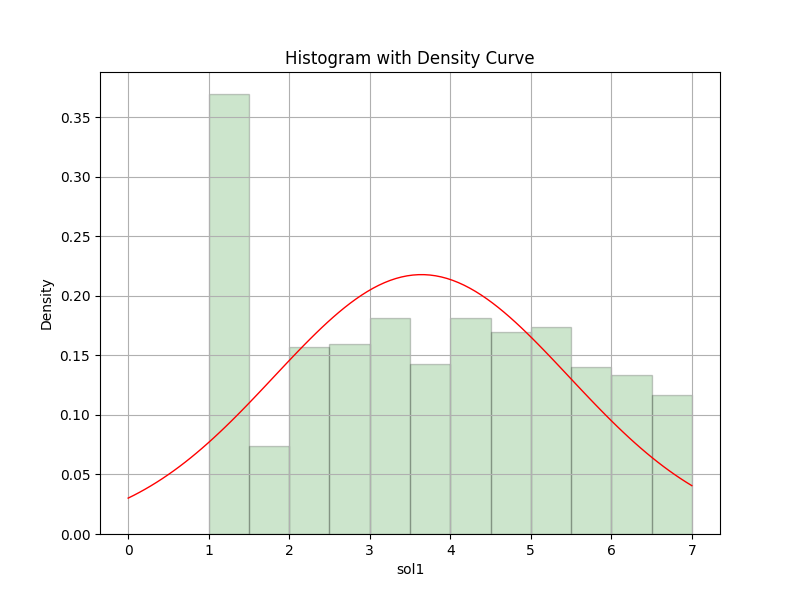
\includegraphics[width=4.06111in,height=2.68611in]{img/histogramaConCurvaDeDensidad.png}
    \caption{Histograma con Curva de Densidad}
    \label{fig:hist_density}%
\end{figure}%

La Figura \ref{fig:hist_density} muestra el histograma con curva de densidad correspondiente a los datos analizados. En el eje Y, se presentan los valores de densidad, mientras que en el eje X, se muestran las notas obtenidas en \textit{sol1}. La mayor concentración de datos se encuentra alrededor del valor 0.35 en el eje Y, lo que indica que la mayoría de las observaciones tienen una nota baja en \textit{sol1}. La curva de densidad, representada en rojo, alcanza su punto más alto entre las notas 3 y 4 en el eje X. Esta curva suavizada muestra la forma general de la distribución de los valores de \textit{sol1}. A medida que las notas aumentan, la densidad disminuye gradualmente.

\subsubsection{Identificación de valores atípicos de la variable objetivo}

La detección de valores atípicos es esencial en el análisis de datos para identificar observaciones que se desvían significativamente de la tendencia general. Estos valores pueden tener un impacto significativo y requerir un análisis más detallado.

A continuación, se muestra una tabla con los valores atípicos identificados mediante el método del Z-score:

\begin{table}[H]
    \centering
    \caption{Valores Atípicos}
    \begin{tabular}{ccccccc}
        \hline
        \textbf{hito1} & \textbf{hito2} & \textbf{exitosos} & \textbf{fallidos} & \textbf{programa} & \textbf{sol1} & \textbf{aprobado} \\
        21.0           & 6.0            & 17                & 14                & UNAB11500         & 1.0           & 0                 \\
        2.0            & 2.0            & 4                 & 27                & UNAB12210         & 1.0           & 0                 \\
        4.0            & 4.0            & 6                 & 41                & UNAB12510         & 1.5           & 0                 \\
        0.0            & 0.0            & 0                 & 47                & UNAB12100         & 1.6           & 0                 \\
        10.0           & 6.0            & 9                 & 38                & UNAB11500         & 1.6           & 0                 \\
        12.0           & 0.0            & 9                 & 38                & UNAB12210         & 2.4           & 0                 \\
        42.0           & 12.0           & 26                & 37                & UNAB21500         & 2.5           & 0                 \\
        32.0           & 32.0           & 26                & 5                 & UNAB11500         & 3.4           & 0                 \\
        9.0            & 0.0            & 7                 & 40                & UNAB11500         & 4.3           & 1                 \\
        38.0           & 6.0            & 28                & 35                & UNAB12210         & 4.4           & 1                 \\
        32.0           & 32.0           & 26                & 5                 & UNAB12210         & 4.6           & 1                 \\
        18.0           & 2.0            & 11                & 20                & UNAB12210         & 4.6           & 1                 \\
        32.0           & 14.0           & 21                & 10                & UNAB12210         & 5.9           & 1                 \\
        13.0           & 25.0           & 16                & 15                & UNAB22115         & 7.0           & 1                 \\
        7.0            & 0.0            & 5                 & 42                & UNAB12100         & 7.0           & 1                 \\
        \hline
    \end{tabular}%
    \label{tab:valores_atipicos}%
\end{table}%

Observando los valores atípicos en la tabla \ref{tab:valores_atipicos}, podemos notar que algunas observaciones difieren significativamente en al menos una de las variables. \say{exitosos} representa las respuestas correctas de la guía, \say{fallidos} indica la cantidad de errores para lograr los \say{exitosos}, \say{programa} se refiere a la carrera a la cual pertenece. \say{sol1} se refiere a la nota obtenida en la solemne, \say{aprobado} se refiere si la nota de solemen es mayor mayor o igual a 4 el alumno es aprobado(columna agregada por medio de script). Estos valores atípicos pueden ser de interés para un análisis más detallado, ya que podrían indicar situaciones excepcionales o errores en la recolección de datos.

\subsection{Comparación de algoritmos}

En esta sección, comparamos varios algoritmos con respecto a nuestras métricas de interés: Accuracy, Precision, Recall y F1 Score (R2). Los algoritmos considerados se dividen en:

% -----------

\subsubsection{Comparacion y Analisis de Modelos de Clasificación}

\begin{itemize}
    \item DecisionTreeClassifier
    \item LogisticRegression
    \item RandomForestClassifier
    \item XGBClassifier
\end{itemize}

Para estos modelos, se utilizará la variable objetivo \say{aprobado}, la técnica \say{Stratified K-Fold Cross-Validation}, ajustaremos el mejor modelo en los datos de entrenamiento y realizaremos predicciones utilizando el mejor modelo.

La mejor configuración para los modelos de clasificación se muestra en el siguiente codigo: \ref{lst:config_clasificacion}:


\begin{lstlisting}[language=Python, caption=Definicion de los Modelos de Clasificación,label=lst:config_clasificacion]
    # Definir los modelos de Clasificacion
    models_clasificacion = [
        DecisionTreeClassifier(
            min_samples_split=10,
            min_samples_leaf=5,
        ),
        LogisticRegression(penalty="l2", C=1.0, solver="lbfgs", max_iter=150),
        RandomForestClassifier(
            max_depth=10,
            min_samples_split=10,
            min_samples_leaf=5,
            random_state=1502,
            n_estimators=500,
        ),
        XGBClassifier(learning_rate=0.1, max_depth=10, n_estimators=150, subsample=1.0),
    ]
\end{lstlisting}

% -----------

\subsubsection{Determinación de Características Clave y Variable Objetivo para Modelos de Clasificación}

En el siguiente fragmento de código, se lleva a cabo el proceso de selección de características relevantes para los modelos de clasificación. La variable objetivo, denominada aprobado, indica si un estudiante ha aprobado o no. Las características seleccionadas, representadas por X, incluyen diversos indicadores y hitos del estudiante, como hito1, hito2, y eventos específicos e0 a e52. Estas características se extraen del dataframe df y se utilizarán para entrenar y evaluar los modelos de clasificación.

\begin{lstlisting}[language=Python, caption=Selección de características y variable objetivo, label=lst:seleccion_caracteristicas]
y = df["aprobado"]
X = df[
['hito1', 'hito2', 'exitosos', 'fallidos','e0', 'e1', 'e2', 'e3', 'e4', 'e5', 'e6', 'e7', 'e8', 'e9', 'e10', 'e11', 'e12', 'e13', 'e14', 'e15', 'e16', 'e17', 'e18', 'e19', 'e20', 'e21', 'e22', 'e23', 'e24', 'e25', 'e26', 'e27', 'e28', 'e29', 'e30', 'e31', 'e32', 'e33', 'e34', 'e35', 'e36', 'e37', 'e38', 'e39', 'e40', 'e41', 'e42', 'e43', 'e44', 'e45', 'e46', 'e47', 'e48', 'e49', 'e50', 'e51', 'e52']
]
\end{lstlisting}

% -----------

\subsubsection{Validación Cruzada Estratificada y Ajuste de Modelos de Clasificación}

En el siguiente fragmento de código, se establece un proceso de validación cruzada estratificada para evaluar varios modelos de clasificación. Primero, definimos las métricas de interés: precisión, exhaustividad, exactitud y la puntuación F1. Luego, aplicamos la técnica de Stratified K-Fold Cross-Validation para garantizar que cada pliegue sea una buena representación del conjunto de datos completo. A continuación, entrenamos cada modelo y evaluamos su rendimiento utilizando las métricas definidas. Finalmente, identificamos y mostramos el modelo con el mejor rendimiento promedio.

\begin{lstlisting}[language=Python, caption=Aplicación de Stratified K-Fold y entrenamiento de modelos, label=lst:stratified_kfold]
    # Definir las métricas
    metrics = ["accuracy", "precision", "recall", "f1"]

    # Realizar Stratified K-Fold Cross-Validation en los datos de entrenamiento y obtener las métricas para cada modelo
    results_train = (
        {}
    )  # Diccionario para almacenar los resultados de entrenamiento de cada modelo

    for model in models_clasificacion:
        model_name = model.__class__.__name__

        cv = StratifiedKFold(n_splits=10, shuffle=True, random_state=1502)
        # Dividir los datos en conjuntos de entrenamiento y prueba
        X_train, X_test, y_train, y_test = train_test_split(
            X, y, test_size=0.2, random_state=1502
        )

        model.fit(X_train, y_train)  # Ajustar el modelo en los datos de entrenamiento
        model_results = (
            {}
        )  # Diccionario para almacenar los resultados de las métricas para el modelo actual

        # Calcular las métricas utilizando validación cruzada
        for metric in metrics:
            scores = cross_val_score(model, X_train, y_train, cv=cv, scoring=metric)
            model_results[metric] = scores

        results_train[
            model_name
        ] = model_results  # Almacenar los resultados del modelo en el diccionario

    best_model = None
    best_score = 0.0

    # Encontrar el mejor modelo basado en la media de las métricas
    for model_name, model_result in results_train.items():
        mean_scores = [np.mean(model_result[metric]) for metric in metrics]
        mean_score = np.mean(mean_scores)

        if mean_score > best_score:
            best_score = mean_score
            best_model = model_name

    # Imprimir el mejor modelo y su puntuación
    print("El mejor modelo en la validación fue:", best_model, best_score)
\end{lstlisting}

% -----------

\subsubsection{Resultados de la Validación Cruzada Estratificada}

Después de aplicar la validación cruzada estratificada y entrenar los modelos de clasificación, se evaluaron sus rendimientos utilizando varias métricas. El modelo que demostró tener el mejor rendimiento promedio fue el RandomForestClassifier, con una puntuación de 0.6433 (redondeado a cuatro decimales). Esta puntuación se calculó como el promedio de las métricas de precisión, exhaustividad, exactitud y la puntuación F1.

Con estos resultados, se destaca la eficacia del modelo de clasificación basado en bosques aleatorios para este conjunto de datos en particular, lo que sugiere que puede ser una opción adecuada para futuras predicciones o análisis relacionados.

\begin{lstlisting}[language=Python, caption=Resultado Mejor modelo en la Validacion de Clasificación, label=lst:rest_bestModelClasification]
    El mejor modelo en la validación fue: RandomForestClassifier 0.6432621955500205
    \end{lstlisting}



% -----------

\subsubsection{Predicciones con el Mejor Modelo en el Conjunto de Prueba}

En el siguiente fragmento de código, buscamos el objeto correspondiente al mejor modelo identificado previamente, en este caso, el RandomForestClassifier. Una vez encontrado, ajustamos este modelo utilizando el conjunto de entrenamiento y luego realizamos predicciones sobre el conjunto de prueba. Posteriormente, calculamos métricas clave, como el Mean Squared Error (MSE) y el R2 Score, para evaluar el rendimiento del modelo en el conjunto de prueba.

\begin{lstlisting}[language=Python, caption=Predicciones y evaluación del mejor modelo, label=lst:prediccion_mejor_modelo]
    best_model_search = None

    # Buscar el objeto del mejor modelo en la lista de modelos
    for model in models_clasificacion:
        if model.__class__.__name__ == best_model:
            best_model_search = model
            break
    
    best_model_search.fit(
        X_train, y_train
    )  # Ajustar el mejor modelo en los datos de entrenamiento
    y_pred = best_model_search.predict(
        X_test
    )  # Realizar predicciones utilizando el mejor modelo
    
    # Calcular y mostrar los resultados obtenidos del mejor modelo
    mse = mean_squared_error(y_test, y_pred)  # Calcular el Mean Squared Error
    r2 = r2_score(y_test, y_pred)  # Calcular el R2 Score
    
    print("Resultados del mejor modelo:", best_model, "en el conjunto de prueba:")
    print("Mean Squared Error:", mse)
    print("R2 Score:", r2)
    \end{lstlisting}

Después de realizar las predicciones con el RandomForestClassifier en el conjunto de prueba, obtuvimos los siguientes resultados:

Mean Squared Error (MSE): 0.3631 (redondeado a cuatro decimales)
R2 Score: 0.4532 (redondeado a cuatro decimales)

Estos resultados proporcionan una medida cuantitativa del rendimiento del modelo en el conjunto de prueba. Es importante notar que un R2 Score negativo indica que el modelo no es adecuado para predecir la variable objetivo en este conjunto de datos, y puede ser menos preciso que un modelo simple que siempre predice el valor medio.

% ------------

\subsubsection{Comparación Gráfica de Métricas de Rendimiento en Modelos de Clasificación (Conjunto de Entrenamiento)}

A continuación, se presentan los resultados obtenidos para el conjunto de entrenamiento. La Figura \ref{fig:metricas_clasificacion} ilustra las métricas de rendimiento de diversos modelos de clasificación evaluados.

\begin{figure}[H]
    \centering
    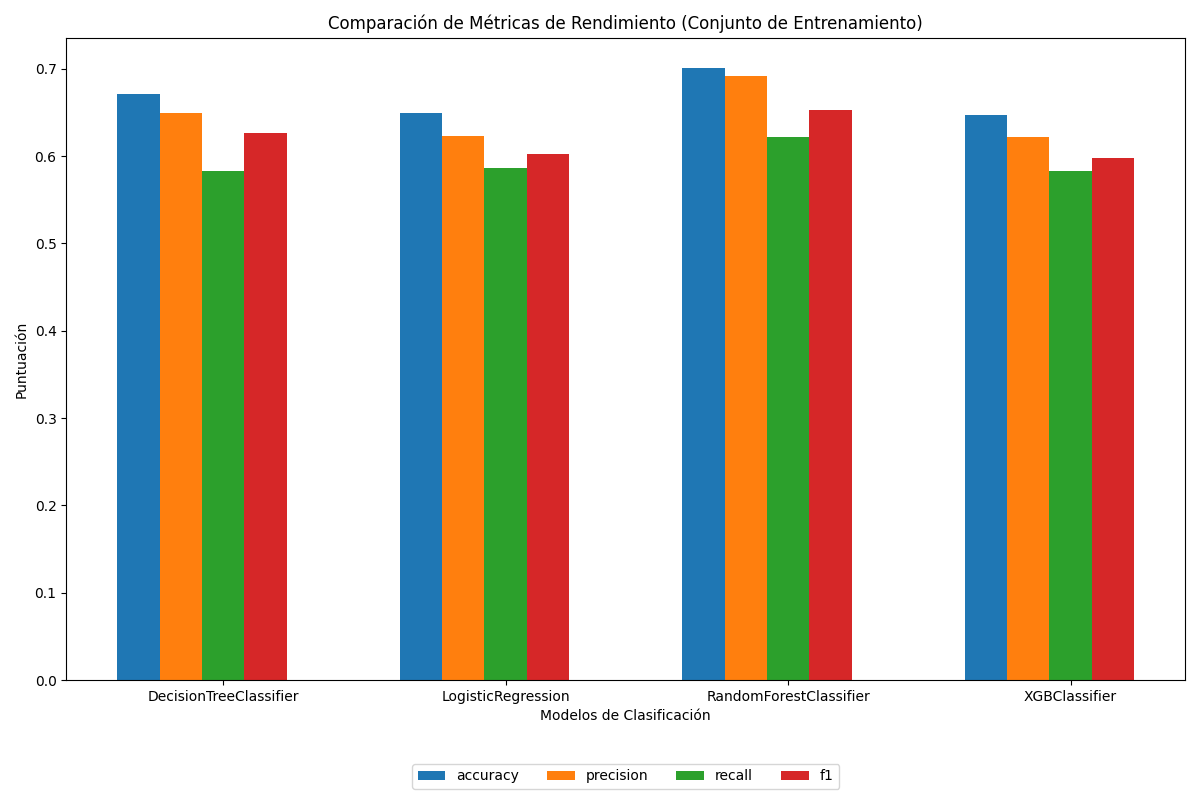
\includegraphics[width=1\textwidth]{img/compara_algoritmos/metricasEntreModelosClasificacion.png}
    \caption{Comparativa de métricas entre modelos de clasificación para el conjunto de entrenamiento.}
    \label{fig:metricas_clasificacion}
\end{figure}

La figura destaca que el modelo RandomForestClassifier sobresale en comparación con los otros modelos en todas las métricas evaluadas. En particular, este modelo logra un F1 Score de 62.53\%, un recall de 58.90\%, una precisión de 67.61\% y una exactitud de 66.54\%.

Para una visión más detallada y estructurada de estos resultados, se presenta la siguiente tabla:

\begin{table}[H]
    \centering
    \caption{Comparación de Métricas de Rendimiento para Modelos de Clasificación}
    \begin{tabular}{lcccc}
        \toprule
        \textbf{Modelo} & \textbf{Accuracy} & \textbf{Precision} & \textbf{Recall} & \textbf{F1} \\
        \midrule
        DecisionTreeClassifier & 0.6409 & 0.6300 & 0.5194 & 0.5708 \\
        LogisticRegression & 0.6617 & 0.6446 & 0.5792 & 0.6069 \\
        RandomForestClassifier & 0.6826 & 0.6761 & 0.5890 & 0.6253 \\
        XGBClassifier & 0.6186 & 0.5865 & 0.5262 & 0.5534 \\
        \bottomrule
    \end{tabular}
    \label{tab:performance_metrics}
\end{table}

Para el conjunto de prueba, los resultados se muestran en la Figura \ref{fig:metricas_clasificacion_bestModel}.

\begin{figure}[H]
    \centering
    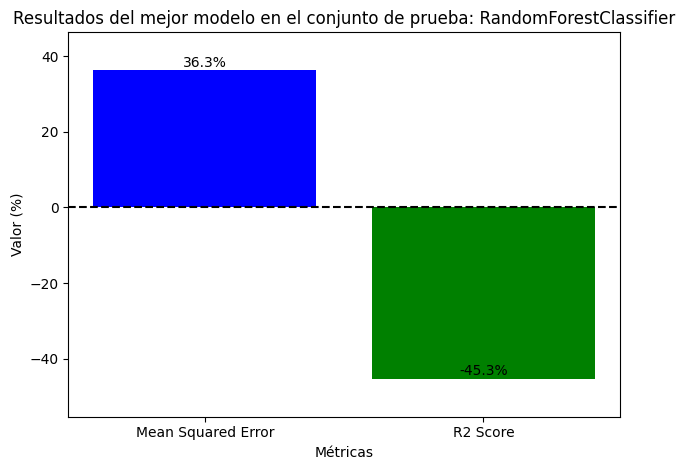
\includegraphics[width=0.8\textwidth]{img/compara_algoritmos/metricasBestModelRandomForesClassifier.png}
    \caption{Métricas del mejor modelo de clasificación en el conjunto de prueba.}
    \label{fig:metricas_clasificacion_bestModel}
\end{figure}

Las métricas cuantitativas para el conjunto de prueba son:

\begin{itemize}
    \item Mean Squared Error: 36.3\%
    \item R2 Score: -45.3\%
\end{itemize}

Con base en los resultados obtenidos, se concluye que el modelo RandomForestClassifier es el más adecuado para abordar este problema de clasificación. En la validación, este modelo demostró ser el mejor, con una puntuación del 62.53\%.

% -----------

\subsubsection{Comparacion y Analisis de Modelos de Regresión}

La regresión es una técnica estadística que permite modelar y analizar las relaciones entre una variable dependiente y una o más variables independientes.

\begin{itemize}
    \item LinearRegression
    \item DecisionTreeRegressor
    \item KNeighborsRegressor
\end{itemize}

Para estos modelos, se utilizará la variable objetivo \say{sol1}, la técnica \say{K-Fold Cross-Validation}, ajustaremos el mejor modelo en los datos de entrenamiento y realizaremos predicciones utilizando el mejor modelo.

La mejor configuración para los modelos de regresión se en el siguiente codigo: \ref{lst:config_regresion}:

\begin{lstlisting}[language=Python, caption=Configuración de los modelos de regresión, label=lst:config_regresion]
# Definir los modelos de regresión
models_regresion = [
    LinearRegression(positive=True, fit_intercept=True),
    DecisionTreeRegressor(
        min_samples_split=5,
        min_samples_leaf=3,
    ),
    KNeighborsRegressor(n_neighbors=8),
]
    \end{lstlisting}

% -----------

\subsubsection{Selección de Características y Variable Objetivo}
Antes de entrenar los modelos, es crucial seleccionar las características que se utilizarán para la predicción y definir la variable objetivo. Esta selección garantiza que los modelos se entrenen con la información más relevante.

\begin{lstlisting}[language=Python, caption=Seleccion de caracteristica y variable objetivo, label=lst:config_varObjetivoCaracteristicas]
# Selección de características y variable objetivo para los modelos de Regresion.
y = df["sol1"]
X = df[
['hito1', 'hito2', 'exitosos', 'fallidos','e0', 'e1', 'e2', 'e3', 'e4', 'e5', 'e6', 'e7', 'e8', 'e9', 'e10', 'e11', 'e12', 'e13', 'e14', 'e15', 'e16', 'e17', 'e18', 'e19', 'e20', 'e21', 'e22', 'e23', 'e24', 'e25', 'e26', 'e27', 'e28', 'e29', 'e30', 'e31', 'e32', 'e33', 'e34', 'e35', 'e36', 'e37', 'e38', 'e39', 'e40', 'e41', 'e42', 'e43', 'e44', 'e45', 'e46', 'e47', 'e48', 'e49', 'e50', 'e51', 'e52']
]
\end{lstlisting}


% -----------
\subsubsection{Validación Cruzada y Entrenamiento}
La validación cruzada es una técnica que permite evaluar la capacidad de generalización de los modelos. En este estudio, se utiliza K-Fold Cross-Validation para entrenar y validar los modelos de regresión en diferentes subconjuntos del conjunto de datos.

\begin{lstlisting}[language=Python, caption=Configuraicones previas antes de la evaluación, label=lst:config_preEval]
# Listas para almacenar los resultados de cada modelo
mse_scores = []
mae_scores = []
r2_scores = []

best_model = None
best_mse = np.inf
best_mae = np.inf
best_r2 = -np.inf

# Colores para los modelos de regresión
colors = ["blue", "green", "red"]
    \end{lstlisting}

% -----------
\paragraph{Evaluación de Modelos de Regresión}
Una vez entrenados, es esencial evaluar el rendimiento de cada modelo. Esta evaluación se basa en métricas específicas que reflejan la precisión y eficacia de los modelos en la predicción de la variable objetivo.

\begin{lstlisting}[language=Python, caption=Codigo de evaluacion de modelos, label=lst:cod_Eval]
# Iterar sobre cada modelo de regresión
for i, model in enumerate(models_regresion):
    # Realizar k-fold cross-validation
    kf = KFold(n_splits=10, shuffle=True, random_state=1502)
    mse_cv_scores = []
    mae_cv_scores = []
    r2_cv_scores = []
    
    for train_index, test_index in kf.split(X):
        # Train-test split para cada fold
        X_train, X_test = X.iloc[train_index], X.iloc[test_index]
        y_train, y_test = y.iloc[train_index], y.iloc[test_index]
        
        # Entrenar el modelo
        model.fit(X_train, y_train)
        
        # Realizar predicciones en el conjunto de prueba
        y_pred = model.predict(X_test)
        
        # Calcular las métricas de evaluación
        mse = mean_squared_error(y_test, y_pred)
        mae = mean_absolute_error(y_test, y_pred)
        r2 = r2_score(y_test, y_pred)
        
        # Almacenar las métricas de evaluación para cada fold
        mse_cv_scores.append(mse)
        mae_cv_scores.append(mae)
        r2_cv_scores.append(r2)
        
    # Calcular la media de las métricas de evaluación para el modelo actual
    avg_mse = np.mean(mse_cv_scores)
    avg_mae = np.mean(mae_cv_scores)
    avg_r2 = np.mean(r2_cv_scores)
    
    # Almacenar las métricas de evaluación para el modelo actual
    mse_scores.append(avg_mse)
    mae_scores.append(avg_mae)
    r2_scores.append(avg_r2)
    
    # Verificar si el modelo actual es el mejor hasta ahora
    if avg_mse < best_mse:
        best_model = model
        best_mse = avg_mse
        best_mae = avg_mae
        best_r2 = avg_r2
    \end{lstlisting}

% -----------

\subsubsection{Resultados y Comparación}
Tras la evaluación, se presentan los resultados obtenidos de cada modelo. Estos resultados permiten identificar qué modelo tiene el mejor rendimiento en términos de precisión y eficacia.

Los resultados obtenidos se presentan en la Figura \ref{fig:metricas_regresion}:

\begin{figure}[H]
    \centering
    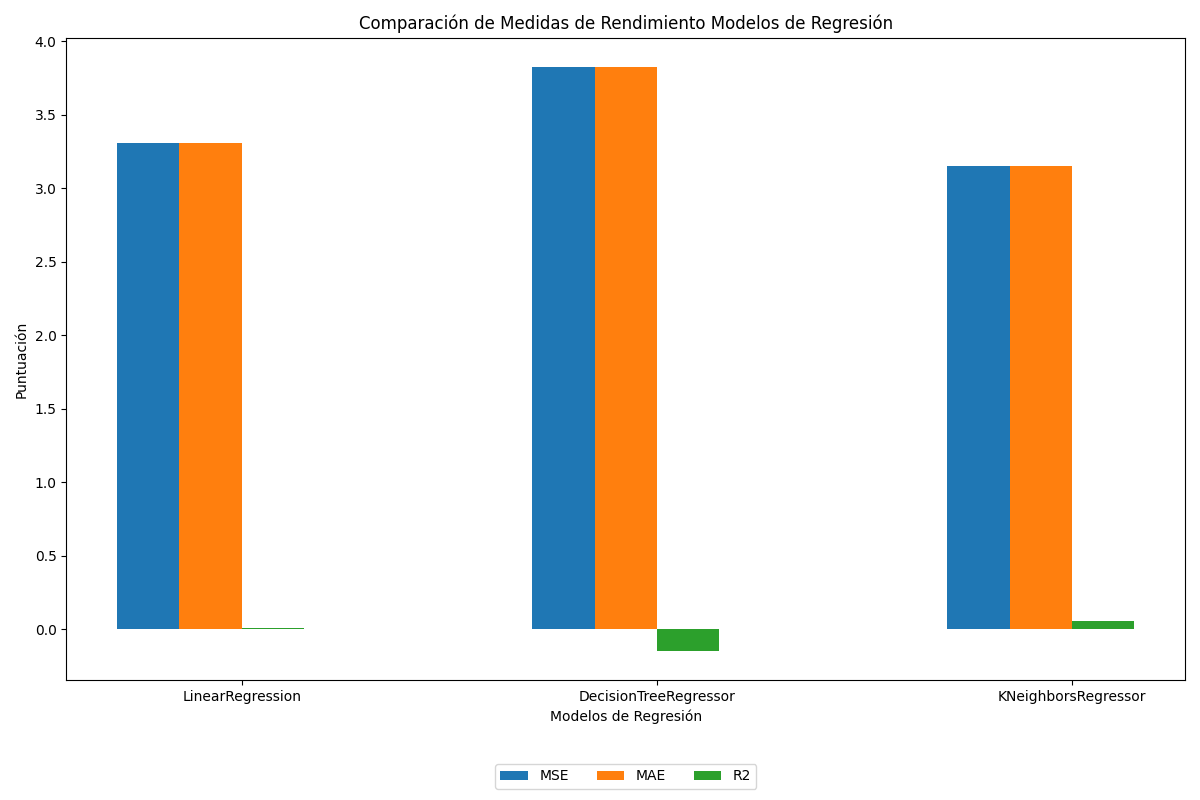
\includegraphics[width=1\textwidth]{img/compara_algoritmos/metricasEntreModelosRegresion.png}
    \caption{Métricas entre modelos de regresión conjunto de entrenamiento}
    \label{fig:metricas_regresion}
\end{figure}

Se observa que el modelo LinearRegression en su conjunto de entrenamiento presenta el comportamiento mas normal utilizando la validacion k-fold cross-validation para variables cuantitativas.

Los resultados sobre el conjunto de prueba se presentan en la figura \ref{fig:metricas_regresion_bestModel}

\begin{figure}[H]
    \centering
    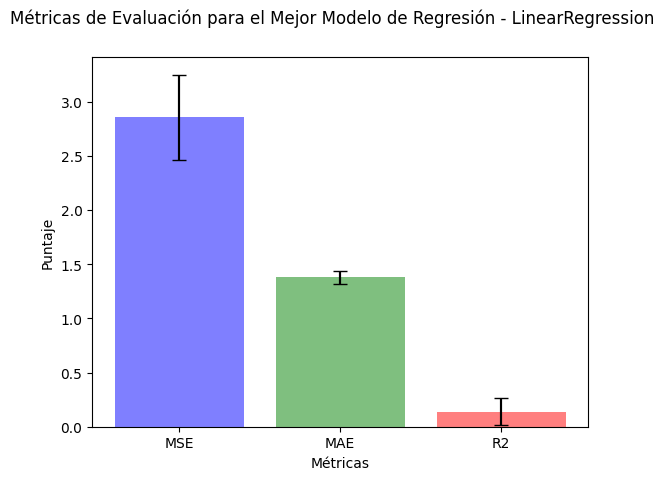
\includegraphics[width=0.7\textwidth]{img/compara_algoritmos/metricasBestModelLinearRegression.png}
    \caption{Métricas Best Model}
    \label{fig:metricas_regresion_bestModel}
\end{figure}

Se observa que el modelo LinearRegression es el mejor modelo de regresión, con un MSE del 3.6\% y un MAE del 1.6\%, valores inferiores a los de los otros modelos evaluados. Además, el modelo LinearRegression presenta un R2 más cercano a 1, con un aumento del 0.1\% en comparación con los demás modelos.

En base en los resultados obtenidos, se puede concluir que el modelo LinearRegression es el más adecuado para problemas de regresion con variable cuantitativas.

\begin{itemize}
    \item El mejor modelo en la validación fue: LinearRegression 14.1\%
\end{itemize}

Resultados del mejor modelo en el conjunto de prueba:

\begin{itemize}
    \item MSE: 3.6.\%
    \item MAE: 1.6\%
    \item R2: 0.1\%
\end{itemize}

% -----------

\subsubsection{Conclusión}

En conclusión, se realizó una comparación exhaustiva de diferentes algoritmos de modelos predictivos para determinar cuál es el más adecuado en términos de origen de datos. Después de analizar y comparar varios algoritmos, se llegó a la conclusión de que el modelo RandomForestClassifier se destaca como el enfoque más efectivo para el origen de datos en cuestión, mientras que el modelo LinearRegression es el más adecuado para análisis de regresión.

\subsection{Analisis SHAP}

Luego de la investigacion realizada en la comparacion de algoritmos realizado y que nos arrojara que el mejor modelo de clasificacion es RandomForestClassifier y de regreseion es LinearRegression, los cuales revisaremos sus resultados.

\subsubsection{Analisis Mejor Modelo Clasificación RandomForestClassifier}
Entrenamiento:

Preparando las coordenadas de análisis X/Y, donde utilizaremos la columna 'aprobado' (binario obtenida de sol1 donde 1 es equivale aprobado con un una nota mayor o igual 4) como referencia para el eje Y, y analizaremos el comportamiento de las demás columnas en relación a dicho eje X.

para comprender mejor los graficos que veremos a continuacion es necesario comprender lo siguiente:
\say{higher} se refiere a las instancias que tienen valores más altos de la característica en comparación con otras instancias, y tienen un mayor impacto en la probabilidad de ser \say{aprobado}. Por otro lado, \say{lower} se refiere a las instancias con valores más bajos de la característica, que tienen un menor impacto en la probabilidad de ser \say{aprobado}.

\begin{figure}[H]
    \centering
    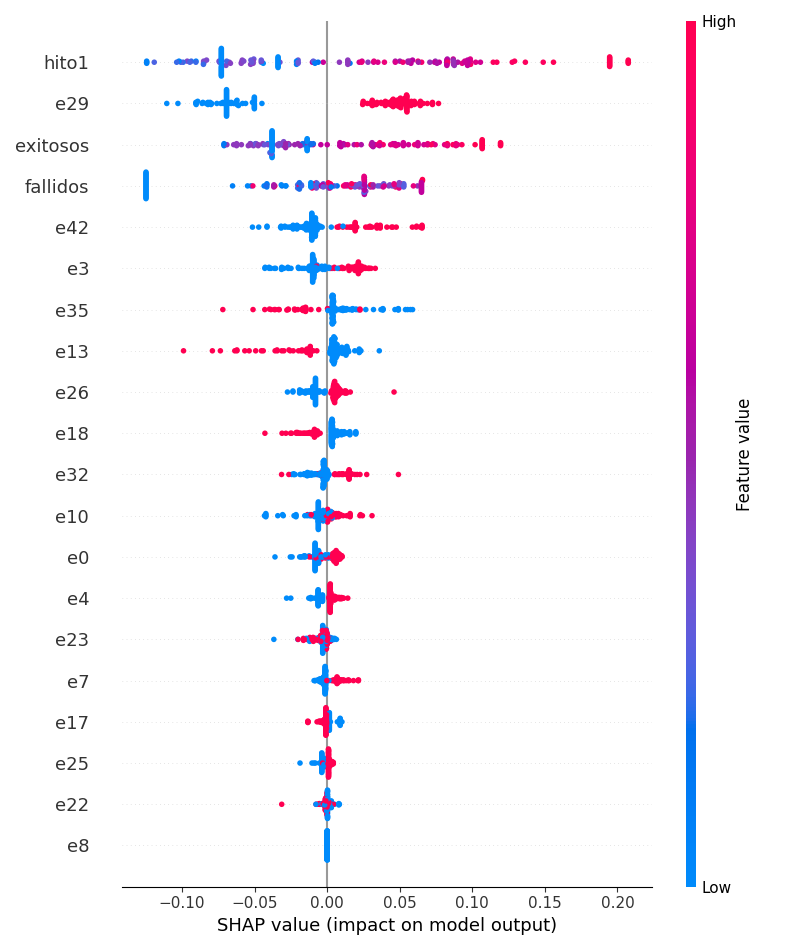
\includegraphics[width=6.0611in,height=6.6861in]{img/shap_rf/shapForcePlot2.png}
    \caption{Característica Variables SHAP}
    \label{fig:caract_var_shap}
\end{figure}

Podemos observar de forma breve que:

\say{hito1} tiene un alto impacto positivo acompañado de 
la pregunta de la guia \say{e29} tambien es una variable de interes de estudio, \say{exitosos} como \say{fallidos} tambien son variables muy interesantes de analisar, ya que estan correlacionadas con la intencion de resolver la guia.

por otro lado tenemos la figura de matplotlib

\begin{figure}[H]
    \centering
    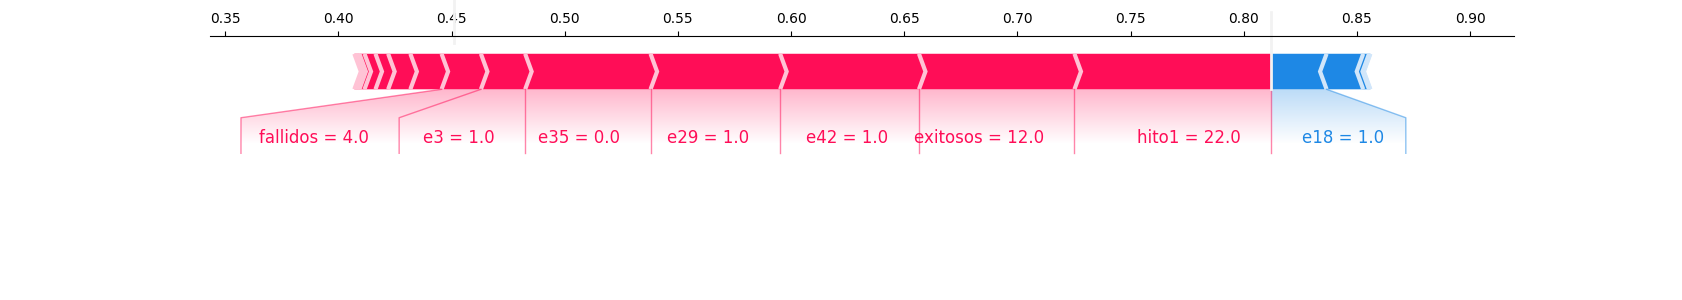
\includegraphics[width=6.0611in,height=1.6861in]{img/shap_rf/shapForcePlot.png}
    \caption{Característica Variables SHAP matplotlib}
    \label{fig:caract_var_shap_mat}
\end{figure}

Al revisar el grafico generado por matplotlib podemos ver:
+ hito1: con un 22.0 cumplido, tiene un 75\%  aproximandamente de importancia.
+ exitosos: tiene 12 respuestas y aproximadamente un 67\% de importancia.
+ e42: La variable tiene una respuesta de 1.0 en la pregunta de la guía y aproximadamente un 59\% de importancia.
+ e29: La variable tiene una respuesta de 1.0 en la pregunta de la guía y aproximadamente un 54\% de importancia.
+ e35: La variable tiene una respuesta de 1.0 en la pregunta de la guía y aproximadamente un 47\% de importancia.
+ e3: La variable tiene una respuesta de 1.0 en la pregunta de la guía y aproximadamente un 46\% de importancia.
+ fallidos: La variable tiene 4.0 intentos para lograr el éxito en la pregunta y aproximadamente un 49\% de importancia.

El impacto más bajo lo presenta la variable \say{e18}, con una respuesta de 1.0 en la pregunta de la guía y una importancia aproximada del 81\% al 85\%.

La marca \say{f(x)} en el gráfico representa el valor de predicción del modelo. En este caso, el valor es 0.81

Graficos de dependencia:

Representa la relación entre los valores de la variable \say{hito1}, say{e29}, say{exitosos},\say{fallidos}, \say{e42} y los valores de Shapley en el modelo. Proporciona una visualización de cómo las variable en cuestion influye en las predicciones del modelo y ayuda a entender su importancia relativa.

\begin{figure}[H]
    \centering
    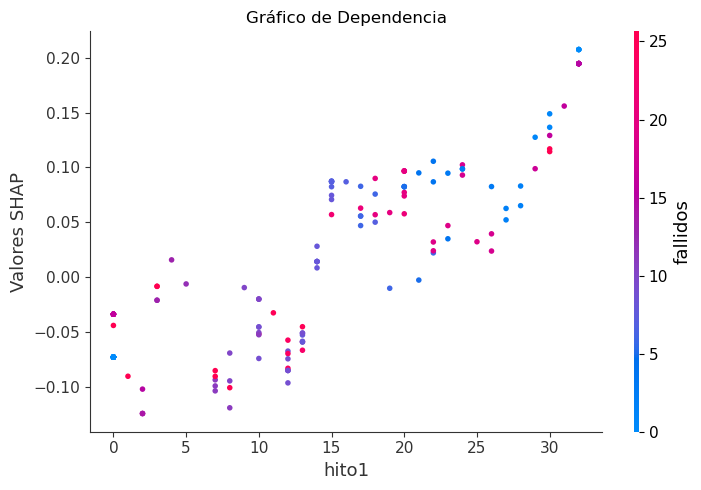
\includegraphics[width=4.0611in,height=2.6861in]{img/shap_rf/hito1.png}
    \caption{Variable dependencia hito1}
    \label{fig:dependencia_hito1}
\end{figure}

\begin{figure}[H]
    \centering
    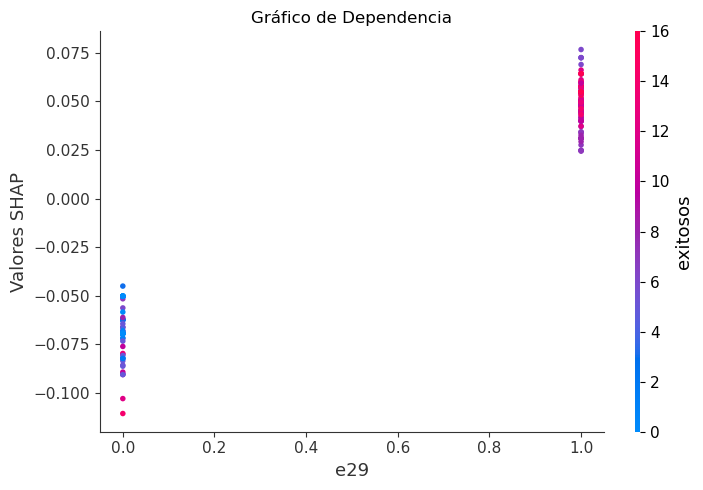
\includegraphics[width=4.0611in,height=2.6861in]{img/shap_rf/e29.png}
    \caption{Variable dependencia e29}
    \label{fig:dependencia_e29}
\end{figure}

\begin{figure}[H]
    \centering
    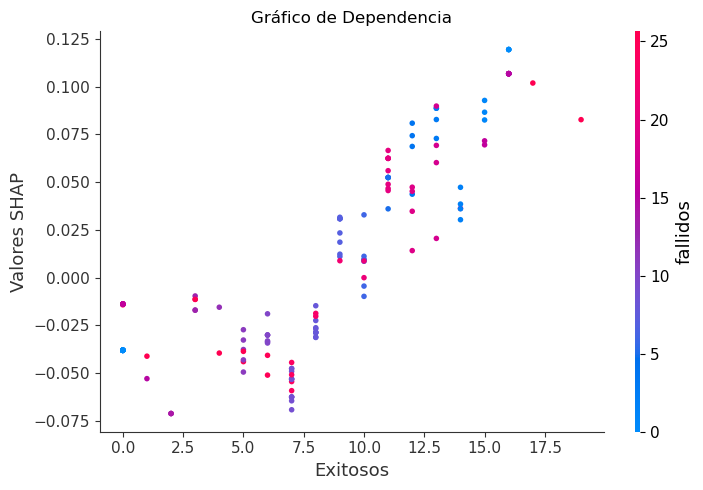
\includegraphics[width=4.0611in,height=2.6861in]{img/shap_rf/exitosos.png}
    \caption{Variable dependencia exitosos}
    \label{fig:dependencia_exitosos}
\end{figure}

\begin{figure}[H]
    \centering
    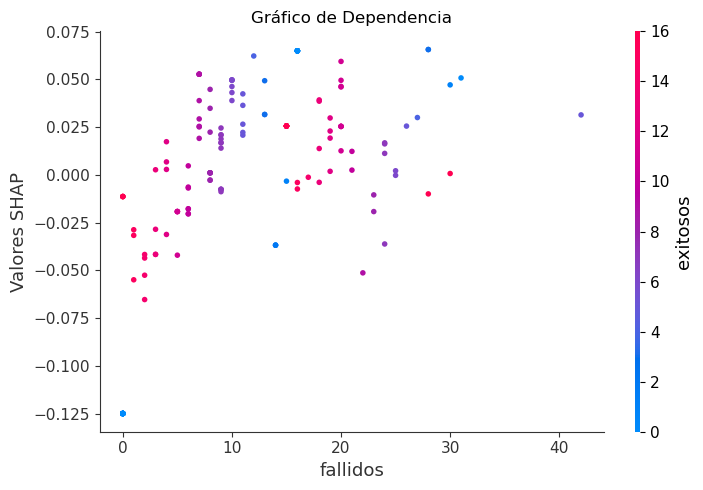
\includegraphics[width=4.0611in,height=2.6861in]{img/shap_rf/fallidos.png}
    \caption{Variable dependencia fallidos}
    \label{fig:dependencia_fallidos}
\end{figure}